\documentclass[10pt,letterpaper]{article}
\usepackage[T1]{fontenc}
\usepackage[utf8]{inputenc}
\usepackage{lmodern}
\usepackage{microtype}
\usepackage[margin=0.78in,top=0.82in,bottom=0.8in,columnsep=0.27in]{geometry}
\usepackage{amsmath,amssymb,booktabs,array}
\usepackage{graphicx}
\usepackage{tikz}
\usetikzlibrary{arrows.meta,positioning,shapes.geometric}
\usepackage[colorlinks=true,urlcolor=blue!60!black,linkcolor=blue!60!black,citecolor=blue!60!black]{hyperref}
\usepackage{fancyhdr}
\usepackage{enumitem}
\usepackage{xcolor}
\usepackage{multicol}
\usepackage{caption}
\setlist[itemize]{leftmargin=*,nosep,topsep=3pt,parsep=1pt}
\setlength{\parindent}{1em}
\setlength{\parskip}{2.2pt}
\setlength{\columnsep}{0.27in}
\pagestyle{fancy}
\fancyhf{}
\fancyhead[L]{\footnotesize SUPER-GENIUS TECHNICAL MANUSCRIPTS}
\fancyhead[R]{\footnotesize NOVEMBER 2026}
\fancyfoot[C]{\thepage}
\renewcommand{\headrulewidth}{0.35pt}
\newcommand{\figstep}[1]{\tikz[baseline=(X.base)]\node[draw=black!55,rounded corners=2pt,fill=black!3,inner sep=5pt,text width=0.85\columnwidth,align=center,minimum height=0.34in] (X) {\footnotesize #1};}
\newcommand{\sourceline}{\vspace{1pt}\noindent\textit{Scope note:} This manuscript presents an architecture and its analysis. A design description is not an empirical security proof.}

\begin{document}

\begin{center}
{\Large\bfseries Wallet-Derived Credentials for Privacy-Preserving\\Crypto-Token Authentication\par}
\vspace{7pt}
{\normalsize Kenneth Hurley\par}
\vspace{2pt}
{\small \url{https://super-genius.github.io}\par}
\vspace{4pt}
{\footnotesize Independent technical manuscript \quad | \quad Version 1.0 \quad | \quad November 1, 2026}
\end{center}
\begin{abstract}
This paper presents a design for authenticating digital-token activity through an existing elliptic-curve wallet while deriving new credentials for private transactions. The architecture combines ECDSA wallet authentication, a key derivation function, ElGamal encryption, proxy addresses, and an optional zero-knowledge proof layer. We describe the intended relationships among account identity, derived credentials, encrypted signatures, and transaction validation. We also identify the security requirements that determine whether a derived credential is secret, recoverable, or linkable to its originating wallet. The paper is a system and protocol design, not a claim that the scheme has undergone formal verification or production security testing.
\end{abstract}
\vspace{3pt}
\noindent\textbf{Keywords:} wallet authentication; deterministic key derivation; ElGamal encryption; zero knowledge; token privacy
\vspace{15pt}
\begin{multicols}{2}

\section{Introduction}
An existing cryptocurrency wallet provides a widely available user credential: possession of the signing key can authorize a message. That capability is useful for services that need transactions, account access, or compute-job payments without requiring users to create a second unrelated identity. A wallet address, however, may also allow transactions to be linked over time.

The design presented here describes a separate cryptographic identity layer for token activity. It begins with ECDSA-based wallet authentication, derives new material through a key derivation function (KDF), creates additional signing or encryption credentials, and considers proxy addresses and zero-knowledge proofs. Its objective is to retain cryptographic authority while reducing the amount of identity and transaction information exposed to observers.

\section{Architecture}
The source design separates the system into ECDSA identity verification, wallet generation, ElGamal key generation, ElGamal encryption, a privacy layer, KDF-based recovery, and optional zk-SNARK integration. These components serve different security goals and should not be collapsed into a single claim of anonymity.

\begin{center}
\begin{minipage}{\columnwidth}
\centering
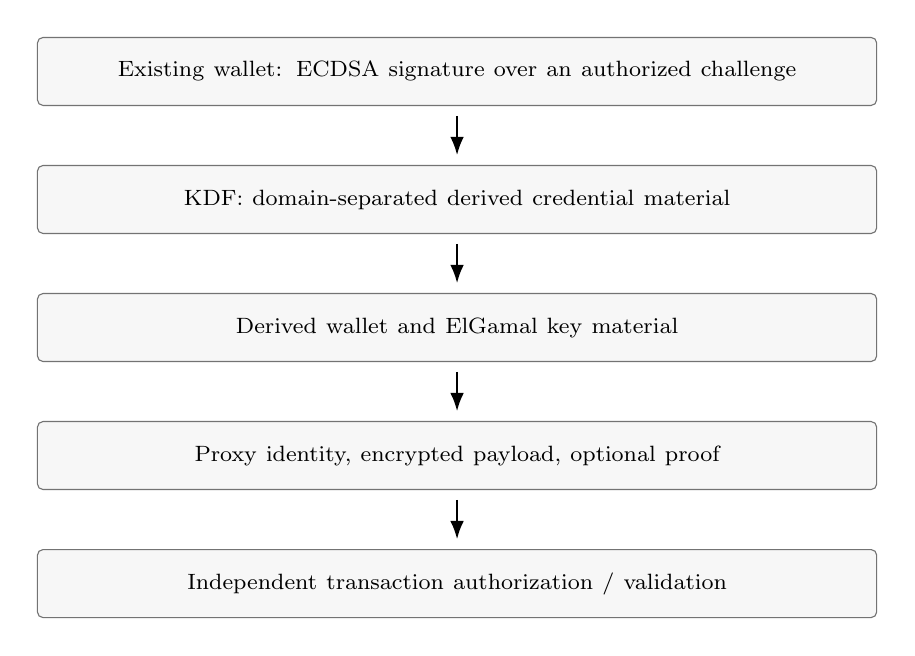
\begin{tikzpicture}[node distance=5mm,>=Latex]
\node (a) {\figstep{Existing wallet: ECDSA signature over an authorized challenge}};
\node[below=of a] (b) {\figstep{KDF: domain-separated derived credential material}};
\node[below=of b] (c) {\figstep{Derived wallet and ElGamal key material}};
\node[below=of c] (d) {\figstep{Proxy identity, encrypted payload, optional proof}};
\node[below=of d] (e) {\figstep{Independent transaction authorization / validation}};
\draw[->,thick] (a.south)--(b.north); \draw[->,thick] (b.south)--(c.north); \draw[->,thick] (c.south)--(d.north); \draw[->,thick] (d.south)--(e.north);
\end{tikzpicture}
\captionof{figure}{Component flow. The diagram shows intended roles; it is not an audited, interoperable wire protocol.}
\end{minipage}
\end{center}

\subsection{Original wallet authentication}
Let $sk_0$ be the original signing key and $pk_0$ its public key. A user signs a challenge $M$:
\begin{equation}
 \sigma=\operatorname{Sign}_{sk_0}(M).
\end{equation}
A relying party uses $pk_0$ to verify the authorization. The challenge should name the application, chain or network, requested operation, recipient, expiration, and a nonce, or it risks cross-service and replay misuse. A signed message proves access to a key, not necessarily a legal-world identity.

\subsection{Derived key material}
The source describes passing a wallet-derived signature or signed ElGamal public value through a KDF to obtain new key material. Abstractly, this is
\begin{equation}
 d=\operatorname{KDF}(\texttt{context},\sigma,\texttt{inputs}).
\end{equation}
The choice of inputs is central to security. If an observer can see $\sigma$ and all other inputs, the observer can calculate $d$ too. Thus a published signature must not, by itself, be the sole source of a derived private key. A safe construction needs adequate secret entropy, domain separation, and careful rules for disclosure.

The derivation must also specify whether signing the same message twice returns identical bytes. Some wallet implementations use different signature encodings or randomized signing. Without canonical output or an explicit seed mechanism, ``regenerate the same key'' is not a portable promise.

\section{Encryption and Proxy Identities}
ElGamal encryption offers public-key encryption with a useful algebraic structure \cite{elgamal}. In a multiplicative group, one ciphertext form for message $m$ and random $r$ is
\begin{equation}
 E_{pk}(m;r)=(g^r,\;m\cdot pk^r).
\end{equation}
The resulting pair is randomized and supports certain homomorphic operations. Encoding small values in a group may allow additive-style relations, but practical decoding and range conditions need care. This property does not grant arbitrary encrypted computation.

The source also proposes proxy addresses derived from new key material. Such addresses may reduce direct use of the original wallet address, but privacy depends on the whole transaction graph. Public funding flows, repeated keys, timing, shared metadata, and proof public inputs can all reintroduce linkability. A proxy address is therefore a pseudonym unless a stronger unlinkability claim is proved.

\section{Optional Zero-Knowledge Authorization}
A zero-knowledge layer could show that a transaction is authorized under an accepted key relation without publishing the underlying key material. A suitable statement might bind the transaction hash, an authorized account commitment, a fresh nonce, and an expiration time. The witness might include a private authorization secret and a valid relation to the commitment.

A proper proof must specify exactly what the verifier learns and what it checks. This includes the arithmetic circuit, public inputs, transcript binding, setup requirements, proving and verification keys, and proof soundness assumptions. The source design identifies zk-SNARK integration as a component, but it does not supply a complete proof circuit or measured prover costs.

\section{Recovery, Rotation, and Compromise}
Deterministic regeneration can reduce key-storage needs, but it creates a tradeoff: the original derivation material becomes highly sensitive. A robust design should consider lost-wallet recovery, compromise of either derived or original keys, and how to revoke old credentials without erasing the audit record.

The source proposes re-encryption of authentication material when an ElGamal key is compromised, followed by an appended update record. A secure implementation must authenticate that rotation request and ensure readers reject the deprecated key. Encrypted data cannot always be recovered from a compromised or lost key; recovery requires a separate trusted recovery path or preserved recovery material.

\section{Threat Model}
The design should be evaluated against attackers who can observe the public chain and pending transactions, replay old signatures, compromise a derived key, or correlate multiple proxy identities. It should also address malicious service endpoints and disclosure of public derivation inputs. Threats from a stolen original wallet key remain particularly serious: derived credentials cannot preserve the original user's authority after the attacker obtains that authority.

\begin{center}
\begin{minipage}{\columnwidth}
\centering\small
\begin{tabular}{p{0.34\columnwidth}p{0.54\columnwidth}}
\toprule
Desired property & Required design evidence\\
\midrule
Reproducible keys & Canonical or stable derivation inputs\\
Secret derived key & Secret entropy absent from public transcript\\
Unlinkable identities & Network and graph-level privacy analysis\\
Authorized transaction & Signature or proof bound to transaction\\
Safe rotation & Revocation semantics and recovery tests\\
\bottomrule
\end{tabular}
\captionof{table}{Claims requiring further evidence before deployment.}
\end{minipage}
\end{center}

\section{MEV and Ordering Limits}
Encrypting transaction details can limit what observers learn before execution. It cannot alone prevent validator reordering, censoring, or other forms of maximal extractable value (MEV). The source design itself contemplates private transaction pools, sequencing choices, time locks, and commit-reveal mechanisms as separate approaches. A token authentication protocol should not claim general MEV protection without specifying those layers and the attacker model.

\section{Potential Role in Decentralized Compute}
A wallet-derived credential layer could authorize prepaid jobs, establish a pseudonymous job account, and provide encrypted authorization metadata while avoiding unnecessary use of the user's primary wallet for every step. The chain, wallet, and compute gateway would each need an explicit rule for which credential can approve spending and which metadata is visible. The proposed design is compatible with investigating such workflows, but this paper does not claim that those integrations have been measured or deployed.

\section{Conclusion}
The described architecture combines existing wallet signatures, key derivation, encryption, proxy credentials, and optional proof verification into a coherent design space. Its promise rests less on the use of any one primitive than on making the trust boundaries and derivation rules precise. The next implementation step is a reproducible message format and a threat-driven review of secrecy, recovery, and linkability.

\end{multicols}
\vspace{6pt}
\begin{thebibliography}{99}

\bibitem{elgamal} T. ElGamal, ``A public key cryptosystem and a signature scheme based on discrete logarithms,'' \emph{IEEE Transactions on Information Theory}, vol. 31, no. 4, 1985.
\bibitem{hkdf} H. Krawczyk and P. Eronen, ``HMAC-based Extract-and-Expand Key Derivation Function (HKDF),'' RFC 5869, 2010.
\bibitem{ecdsa} National Institute of Standards and Technology, ``Digital Signature Standard (DSS),'' FIPS 186-5, 2023.
\bibitem{eip712} Ethereum Improvement Proposal 712, ``Typed structured data hashing and signing,'' Ethereum EIPs.
\bibitem{zk} E. Ben-Sasson et al., ``Succinct non-interactive zero knowledge for a von Neumann architecture,'' \emph{USENIX Security}, 2014.
\bibitem{source} Author-supplied technical design specification for cryptographic token authentication, 2025.

\end{thebibliography}
\vspace{6pt}
\noindent\rule{\textwidth}{0.3pt}
\noindent\footnotesize Prepared for publication at \url{https://super-genius.github.io}. This work is a technical exposition, not a claim of independent certification or completed performance evaluation.
\end{document}
